\section{Distinguish Devices}
IoT applications utilise a great variation of devices, with each having different processing power. This implies that the processing time of some specific packets can be exploited as a hint to the model of device. 

PING is therefore an ideal feature supported in 6LoWPAN that can be exploited to perform such an attack due to:
\begin{enumerate}
	\item PING is processed in a standardised routine where nearly no computation is required, minimising the noise in the data.
	\item The support of PING is required by the IPv6\cite{rfc4443}, making the attack universally applicable.
\end{enumerate}

\subsection{Contiki MAC}\label{TimingWithContikiMAC}
Contiki adopts a Radio Duty Cycle (RDC) protocol called Contiki MAC\cite{ContikiMAC} to preserve energy. Briefly speaking, Contiki MAC works by switching off the radio for most of the times but periodically wakes up for a short period for signal detection, and keeps the radio up only if a signal is detected. On the other hand, the sender repeats the signal when sending a packet, until a receiver acknowledges the sender or time out.

As a result, duplicated packets may be observed in the captured traffic. To best approximate the processing time for a specific PING request, the PING Response Interval (PRI) is defined as the time elapsed between the last PING request being sent and the first PING response being replied. 

\paragraph{Example}
\Cref{PRIExample} shows an example of packets captured by Wireshark\cite{Wireshark}. 6 duplicated PING requests, \#$970$ to \#$975$, are replied by a single response, \#$977$, matched by their \textit{seq} values($18$). The PRI is therefore computed as their difference in time which is:
\begin{equation*}
PRI = 74.874242 - 74.786970 = 0.087272(s) = 87.272(ms)
\end{equation*}

\AddFigure{fig/PRI.png}{PRI Example}{PRIExample}

\subsection{Pinging Different Devices}
We measured the PRI for two devices, TelosB\cite{TelosB} and CC2538\cite{CC2538}. Optionally for TelosB, the default software AES implementation can be replaced a hardware coprocessor. We demonstrate our result of PRIs on the above platforms in \Cref{PINGTiming}.

\begin{figure}[ht!]
	\centering
	\begin{subfigure}{0.4\textwidth}
	{
		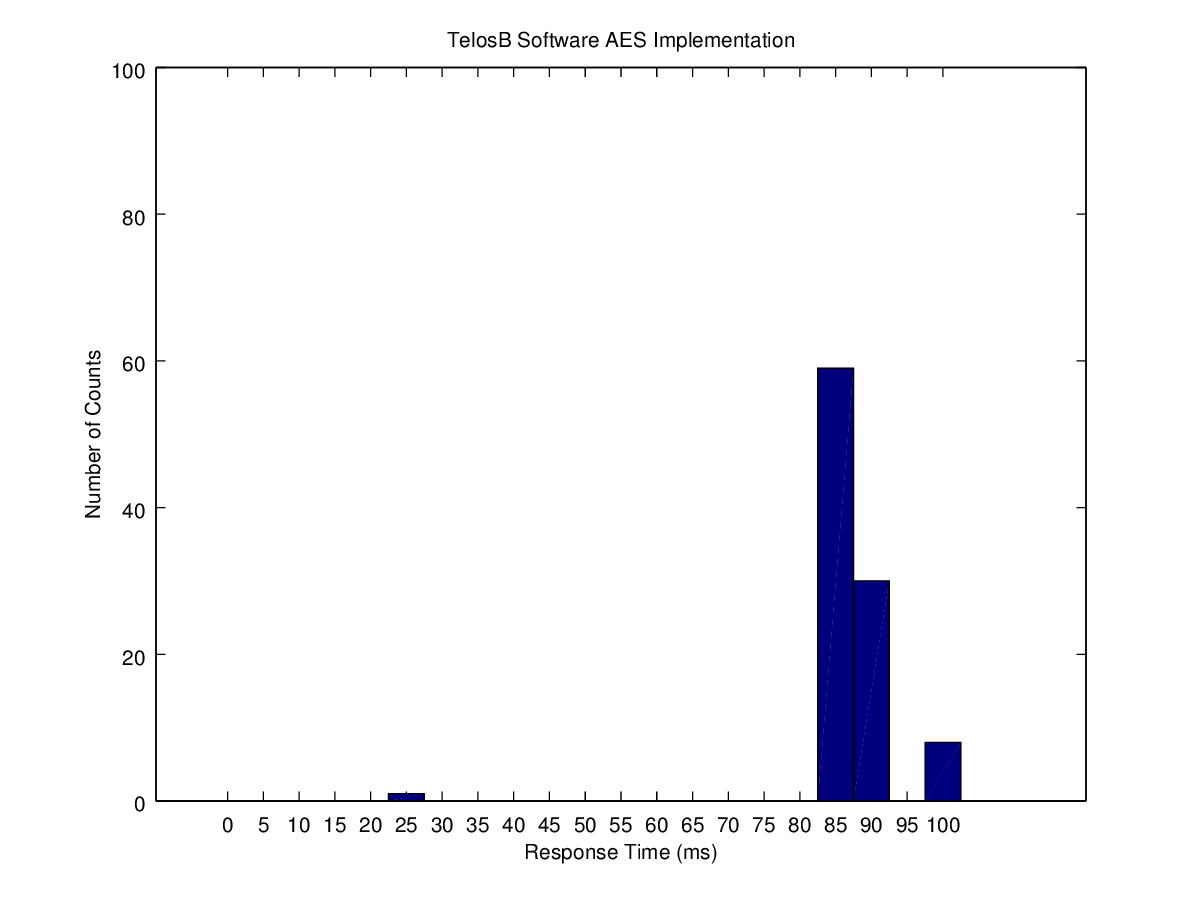
\includegraphics[width=\textwidth]{fig/noncoresec_ping_telosb_sw.png}
	}
	\end{subfigure}
	\begin{subfigure}{0.4\textwidth}
	{
		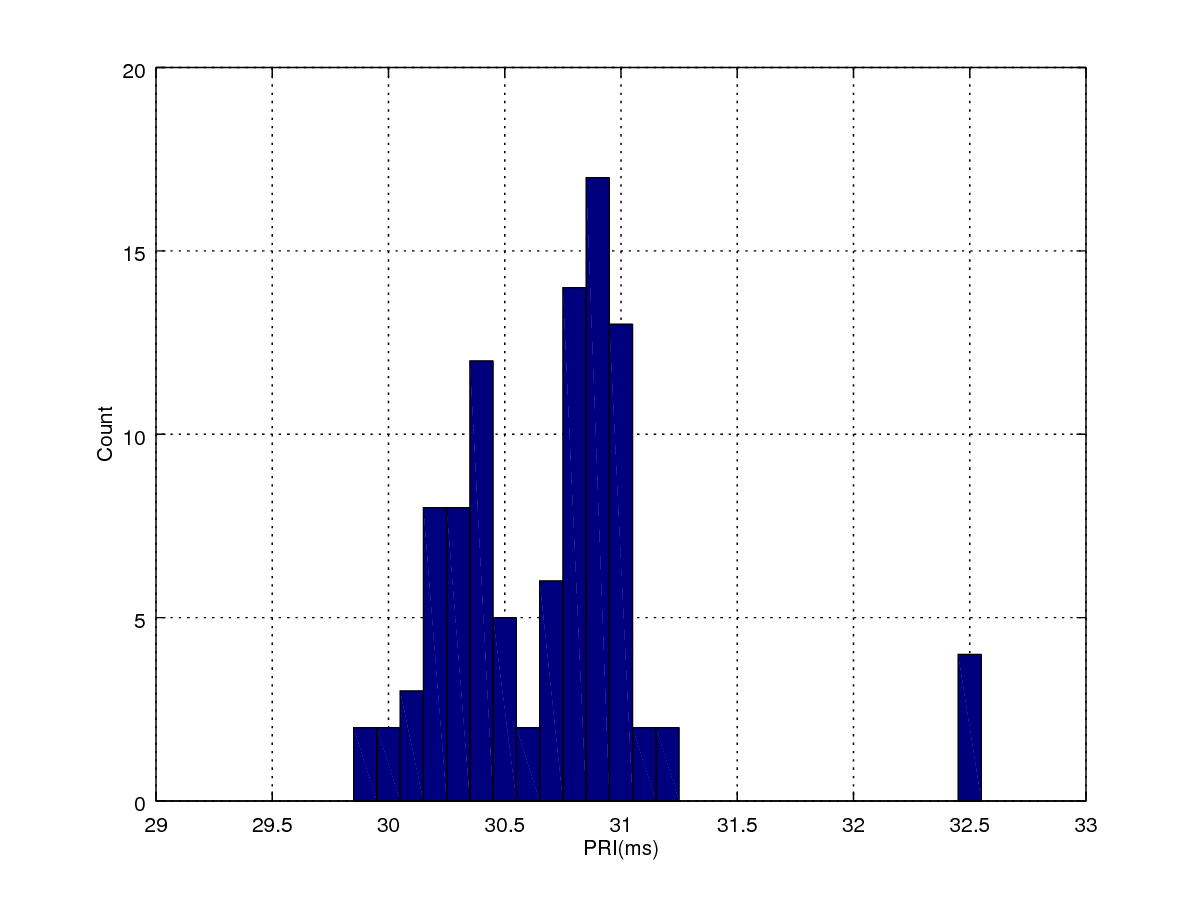
\includegraphics[width=\textwidth]{fig/noncoresec_ping_telosb_hw.png}
	}
	\end{subfigure}
	\begin{subfigure}{0.4\textwidth}
	{
		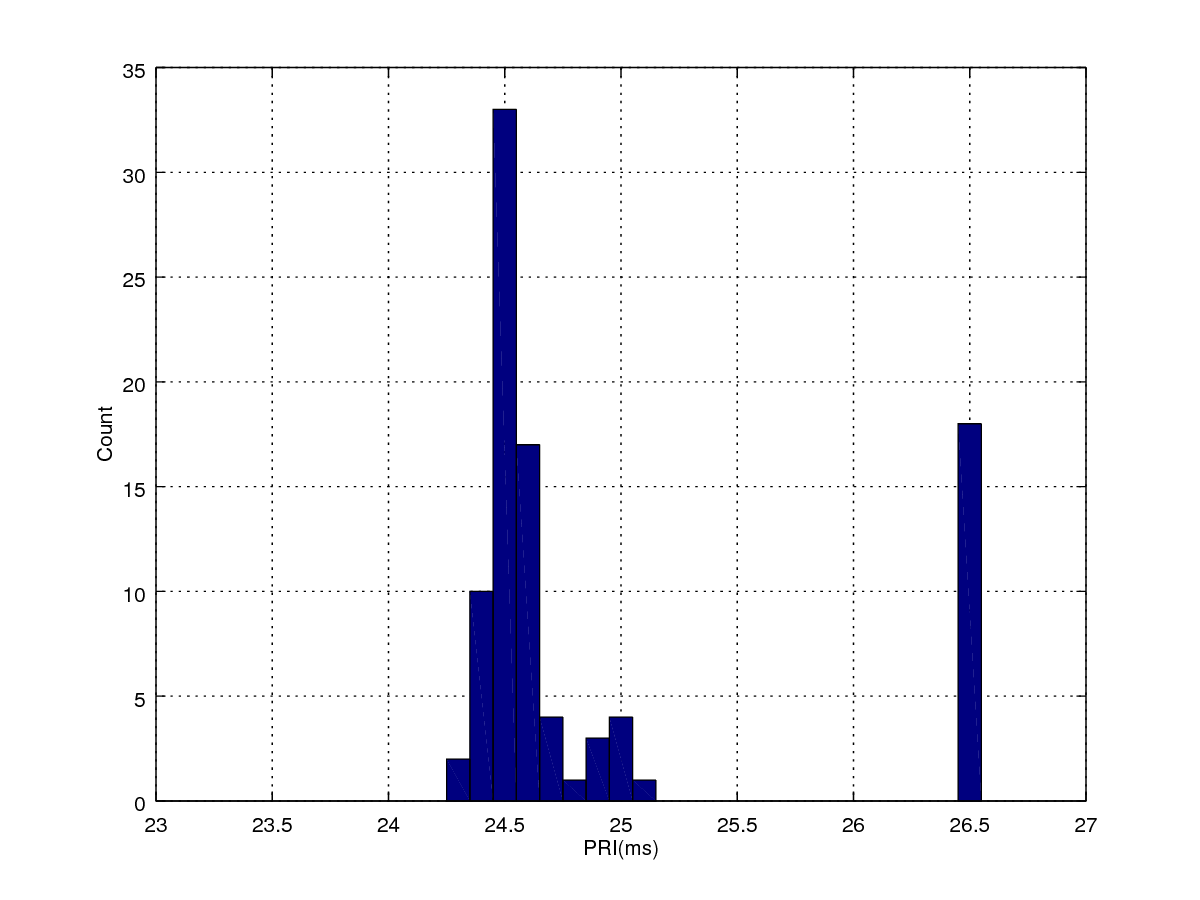
\includegraphics[width=\textwidth]{fig/noncoresec_ping_cc2538_sw.png}
	}
	\end{subfigure}
	\caption{PING Reponse Time for TelosB and CC2538\label{PINGTiming}}
\end{figure}

%Data Analysis
Observing \Cref{PINGTiming}, it is intuitively clear that different devices (and setups) result into different PRIs. However, we also realised that certain outliers exist in the data, usually significantly greater than $100ms$. A common cause of outliers could be that the CPU was occupied by other tasks when the PING request is received and thus delaying the response. 

Not to our surprise, the means and medians are significantly different to each others, as we summarised in \Cref{PINGResponseTimeTbl}. We consider the median as a statistically more effective indicator as it is less affected by the outliers. 

\begin{table}[ht!]
	\centering
	\adjustbox{max width = \textwidth}
	{
		\begin{tabular}{|c|c|c|}
			\hline
			              & Mean (ms)     & Median (ms)   \\ \hline
			TelosB HW AES & 37.20 & 30.77 \\ \hline
			TelosB SW AES & 105.19        & 87.40          \\ \hline
			CC2538 SW AES & 48.83         & 24.55          \\ \hline
		\end{tabular}
	}
	\caption{PING Response Time}
	\label{PINGResponseTimeTbl}
\end{table}

The result indicates that it would be possible to reveal device models (and setups) from the encrypted traffic by simply compare PRIs to profiled data, assuming they are selected from a known set. Combined with the attack in \Cref{ICMPAttack}, one could further apply the similar timing attack on any extractable ICMP messages in the encrypted traffic.